%%%%%%%%%%%%%%%%%%%%%%%%%%%%%%%%%%%%%%%%%
% Engineering Calculation Paper
% LaTeX Template
% Version 1.0 (20/1/13)
%
% This template has been downloaded from:
% http://www.LaTeXTemplates.com
%
% Original author:
% Dmitry Volynkin (dim_voly@yahoo.com.au)
%
% License:
% CC BY-NC-SA 3.0 (http://creativecommons.org/licenses/by-nc-sa/3.0/)
%
% Modificaciones por Roberto Cerdas
%
% Si desea utilizar notas al margen, favor leer los comentarios en las líneas 32 y % 52. Si desea colocar un logo, favor leer comentario en línea 54. El comando     % \marginnote{texto} introduce notas al margen.  
%
%%%%%%%%%%%%%%%%%%%%%%%%%%%%%%%%%%%%%%%%%

%----------------------------------------------------------------------------------------
%	PACKAGES AND OTHER DOCUMENT CONFIGURATIONS
%----------------------------------------------------------------------------------------

\documentclass[12pt,a4paper]{article} % Use A4 paper with a 12pt font size - different paper sizes will require manual recalculation of page margins and border positions

\usepackage[spanish]{babel} % Utilizar reglas de idioma español
\usepackage[utf8]{inputenc} % Use UTF-8 encoding
\usepackage{marginnote} % Required for margin notes
\usepackage{wallpaper} % Required to set each page to have a background
\usepackage{lastpage} % Required to print the total number of pages
%\usepackage[left=1.3cm,right=4.6cm,top=1.8cm,bottom=4.0cm,marginparwidth=3.4cm]{geometry} % Comentar la línea abajo y descomentar esta para usar notas al margen
\usepackage[left=1.3cm,right=1.3cm,top=1.8cm,bottom=4.0cm]{geometry} % Adjust page margins
\usepackage{amsmath} % Required for equation customization
\usepackage{amssymb} % Required to include mathematical symbols
\usepackage{xcolor} % Required to specify colors by name
\usepackage[square, comma, sort&compress]{natbib} % Use the natbib reference package - read up on this to edit the reference style; if you want text (e.g. Smith et al., 2012) for the in-text references (instead of numbers), remove 'numbers' 

\usepackage{fancyhdr} % Required to customize headers
\setlength{\headheight}{80pt} % Increase the size of the header to accommodate meta-information
\pagestyle{fancy}\fancyhf{} % Use the custom header specified below
\renewcommand{\headrulewidth}{0pt} % Remove the default horizontal rule under the header

\setlength{\parindent}{0cm} % Remove paragraph indentation
\newcommand{\tab}{\hspace*{2em}} % Defines a new command for some horizontal space

\newcommand\BackgroundStructure{ % Command to specify the background of each page
\setlength{\unitlength}{1mm} % Set the unit length to millimeters

\setlength\fboxsep{0mm} % Adjusts the distance between the frameboxes and the borderlines
\setlength\fboxrule{0.5mm} % Increase the thickness of the border line
\put(10, 10){\fcolorbox{black}{white!10}{\framebox(192,247){}}} % Main content box
%\put(165, 10){\fcolorbox{black}{blue!10}{\framebox(37,247){}}} % Margin box: Descomentar para utilizar notas al margen.
\put(10, 262){\fcolorbox{black}{white!10}{\framebox(192, 25){}}} % Header box
%\put(143, 263){\includegraphics[height=23mm,keepaspectratio]{logo}} % Logo box - maximum height/width: 25x42. Descomentar esta línea para usar logo.
}

%----------------------------------------------------------------------------------------
%	HEADER INFORMATION
%----------------------------------------------------------------------------------------

\fancyhead[L]{\begin{tabular}{l r | l r} % The header is a table with 4 columns
\textbf{Proyecto} & Diseño flip-flop CMOS & \textbf{Página} & \thepage/\pageref{LastPage} \\ % Project name and page count
\textbf{Trabajo} & Proceso de diseño & \textbf{Actualizado en:} & 31/10/2015 \\ % Job number and last updated date
\textbf{Curso} & VLSI & \textbf{Revisado en:} & 2/11/2015 \\ % Version and reviewed date
\textbf{Diseñador} & López F. - Quirós.J.& \textbf{Revisado por:} & Alfonso Chacón Rodríguez \\ % Designer and reviewer
\end{tabular}}

%----------------------------------------------------------------------------------------

\begin{document}



\AddToShipoutPicture{\BackgroundStructure} % Set the background of each page to that specified above in the header information section

%----------------------------------------------------------------------------------------
%	DOCUMENT CONTENT
%----------------------------------------------------------------------------------------


\section{Resumen} 

En este documento se presentan los resultados del diseño de un registro flip-flop en una tecnología ON Semiconductor 0.5 $\mu$m, el cual se caracterizó y se midieron sus valores de tiempo mas importantes. Tambien se presenta las respuesta a las preguntas de teoriía sobre los valores de tiempo en un registro flip-flop y sobre las diferencias entre los flip-flop estáticos y dinámicos.

\section{Introducción} 

El flip-flop es un tipo de circuito secuencial, capaz almacenar un valor lógico a partir de su entrada en un flanco de señal de reloj. Esta señal perdura durante el periodo de la señal de reloj hasta el proximo flanco de subida o de bajada, dependiendo de su fabricación. Idealmente, el tiempo requerido para el almacenamiento de información es cero, pero a como veremos a continuación, dependerá de la tecnología con la que se ha constrido el flip-flop que habrán tiempos que se deberán respetar para que su funcionamiento sea el esperado.

Para este documento se iniciará dando una breve explicación acerca de lo que son los tiempos que estarán definidos para el diseño del flip-flop incluidos los tiempos de propagación de la señales. Luego se explicarán acerca de lo que son los registros estáticos y dinamico, asi como las ventajas y desventajas que poseen cada uno, esto con el fin de observar el potencial que poseen cada uno en diversas aplicaciones.

También se mostrará en este documento, el diseño en layout de un flip-flop master-slave para 1 bit en tecnología ON-semiconductor 0.5 $\mu$m. asi como las consideraciones que se tomaron para el mismo.

Por último se mostrará las simulaciones que se realizaron para la caracterización del flip-flop y medición de los valores de tiempos del mismo.

\section{Definición de conceptos}

\begin{itemize}
\item Set-up time: Es el tiempo mínimo el cual debe tener la entrada D antes del flanco de reloj, para que sea un valor válido de entrada y pueda ser cargado en el flip-flop. 
Para el circuito propuesto, esta propagación es medible por los tiempos de propagación que requiere los transistores del bloque Master, esto antes del flanco de reloj y que se empiece a propagar la entrada en el bloque Slave. De no ser así los valores de los buffers de salida del bloque no se traslapen y den un valor incorrecto. 
El valor de set-up en un flip-flop master salve es el mostrado en la ecuación (), esta viene de que la entrada debe propagarse en 3 inversores y en 1 buffer de paso:

\begin{equation}\label{eqn:set_up}
F=3 *tpd _{inv} + tpd _{tx}
\end{equation}

\item Hold time: Es el tiempo mínimo el cual se debe mantener el valor de entrada D, luego del flanco de reloj, para que sea un válido que se pueda cargar en el flip-flop.
Para el circuito propuesto, este valor es cero. Esto porque al haberse dado el flanco de reloj, el transistor de paso en la entrada en el bloque Master se cierra por lo que el valor de entrada a partir de ese momento no afectará en lo absoluto a la salida. 

\item Tiempo de propagación: Es el tiempo que le toma al flip-flop en el peor caso, para tener un valor válido de salida igual al valor cargado leído en la entrada.
En el Flip-Flop Master-Slave, este tiempo es el cual le tomará la salida del bloque master propagarse en el bloque Slave. Para ello solo le tomará el tiempo de propagación de un inversor y de un buffer de paso, ya que se consideró en el setup-time el tiempo para el transistor de entrada del bloque.
Este valor se puede calcular con la ecuación (): 

\begin{equation}\label{eqn:propagacion}
F=tpd_{tx} + tpd_{inv}
\end{equation}

\item Tiempo de contaminación: Es el menor tiempo que le toma al flip-flop para tener un valor de salida igual al valor de la entrada que se había leído anteriormente.

\end{itemize}

\section{Flip-Flops estáticos y dinámicos}


Los registros estáticos son aquellos que pueden mantener su salida mientras haya alimentación en el circuito. Estos son retroalimentados entre la salida y la entrada del registro para mantener constante la tensión en la salida y que no haya fluctuaciones.  
Estos registros se usan en componentes que no requieren rápidos cambios en su valor almacenado o que necesitan un almacenamiento por largo periodo de tiempo. Ejemplo de ello son registros que se les deben cargar la configuración del funcionamiento del circuito.

Los registros dinámicos son el complemento de los estáticos. La duración de su valor almacenado es de poca duración ya que el valor es cargado en las capacitancias parásitas del registro y este se irá disipando con respecto al tiempo. Este registro es de alta velocidad y baja disipación de potencia por lo que es muy usado en registro de pipeline y de transmisión de datos donde se requiere que haya una rápida carga de los datos.


\section{Diseño del layout}

En esta sección se presentará y explicará el diseño en layout de un flip-flop Master-Slave para 1 bit el cual deberá soportar una carga de FO4. Se explicará cada módulo creado en la herramienta Electric y se mostrará el circuito completo.

Para los bloques Master, Slave y el inversor conectado entre ellos se hizo la dimensión de los transistores a partir de los valores medidos en la Tarea 1, mientras que el último inversor se dimensionó con respecto a la carga que debe soportar el flip-flop. El pitch usado es el que se encontró en la Tarea 2. 

\subsection{Bloque Master}

Es el segmento de entrada delflip-flop. El esquematico es el mostrado en la figura \ref{fig:Master_s} y el layout es el mostrado en la figura \ref{fig:Master_l}. Fue posible reducir bastante su largo creándolo de esta forma y separando el inversor de salida en un módulo aparte. 

\begin{figure}[htbp]
  \centering
    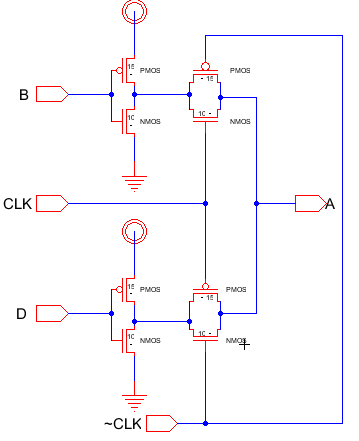
\includegraphics[scale=0.45]{./Master_s.png}
    \rule{35em}{0.5pt}
  \caption[Master]{Esquemático del segmento del Bloque Master}
  \label{fig:Master_s}
\end{figure}

\begin{figure}[htbp]
  \centering
    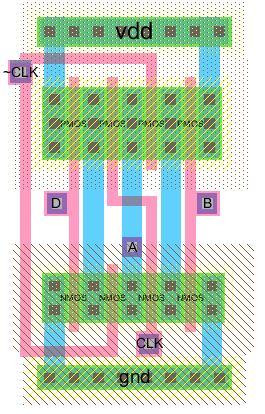
\includegraphics[scale=0.6]{./Master_l.png}
    \rule{35em}{0.5pt}
  \caption[Master]{Layout del segmento del Bloque Master}
  \label{fig:Master_l}
\end{figure}

\subsection{Inversor en el Master}

Este módulo es solamente un inversor de transistores de tamaño mínimo, que viene incluido en el módulo Master. Su esquemático es el mostrado en la figura \ref{fig:Inv_s} y su layout es el de la figura \ref{fig:Inv_l}.

\begin{figure}[htbp]
  \centering
    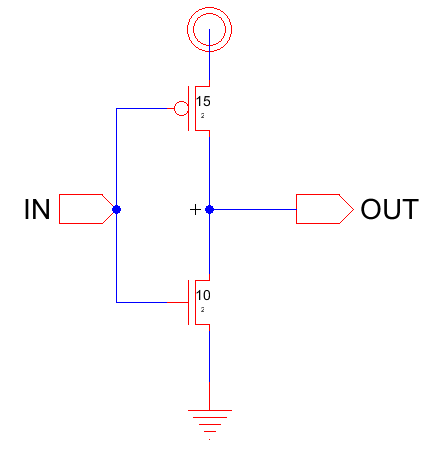
\includegraphics[scale=0.45]{./Inv_s.png}
    \rule{35em}{0.5pt}
  \caption[Inv]{Esquemático del inversor de salida del bloque Master}
  \label{fig:Inv_s}
\end{figure}

\begin{figure}[htbp]
  \centering
    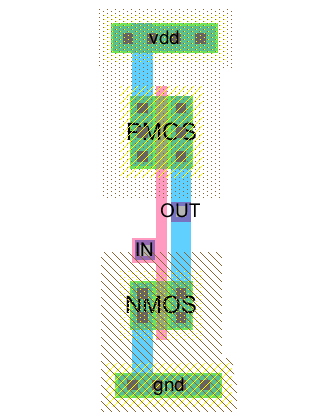
\includegraphics[scale=0.6]{./Inv_l.png}
    \rule{35em}{0.5pt}
  \caption[Inv]{Layout del inversor de salida del bloque Master}
  \label{fig:Inv_l}
\end{figure}

\subsection{Bloque slave}

El tercer módulo del circuito presenta mucha similitud con el módulo Master, como se presenta en las figuras de esquemático (figura \ref{fig:Slave_s}) y de layout (figura \ref{fig:Slave_l}) con la diferencia del cambio de las señales de control de los relojes y el posicionamiento de los conectores para usar menos metal 2.

\begin{figure}[htbp]
  \centering
    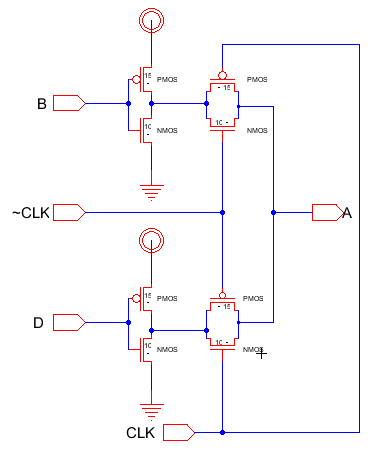
\includegraphics[scale=0.45]{./Slave_s.png}
    \rule{35em}{0.5pt}
  \caption[Slave]{Esquemático del segmento del Bloque Slave}
  \label{fig:Slave_s}
\end{figure}

\begin{figure}[htbp]
  \centering
    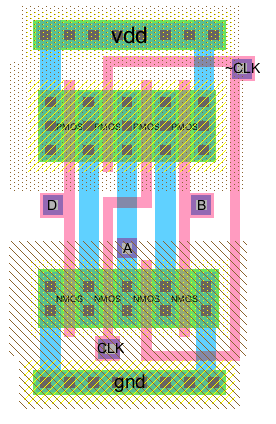
\includegraphics[scale=0.6]{./Slave_l.png}
    \rule{35em}{0.5pt}
  \caption[Slave]{Layout del segmento del Bloque Slave}
  \label{fig:Slave_l}
\end{figure}

\subsection{Buffer inversor de salida}

Este inversor de salida se hizo a partir de los calculos empleados para un dimensioamiento de ancho para soportar una carga de FO4. Se tiene como resultado que el ancho para el transistor PMOS es de 60$\lambda$ mientras que para el NMOS es de 40$\lambda$.
Por cuestiones de dimensionamiento en el layout, este módulo es muy ancho para ajustarse a los demás, por lo que se optó por crear diversos inversores de menor tamaño, pero que puedan soportar la misma carga y tengan un funcionamiento similar al diseñado anteriormente. De esta forma se obtiene como resultado el módulo mostrado en las figuras \ref{fig:FO4_s} de esquemático y \ref{fig:FO4_l} de layout.

\begin{figure}[htbp]
  \centering
    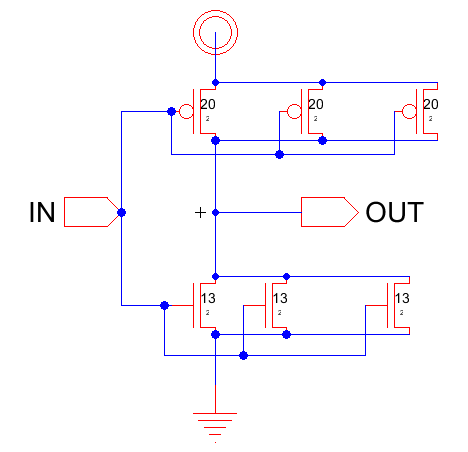
\includegraphics[scale=0.45]{./FO4_s.png}
    \rule{35em}{0.5pt}
  \caption[FO4]{Esquemático del inversor de salida del bloque Slave}
  \label{fig:FO4_s}
\end{figure}

\begin{figure}[htbp]
  \centering
    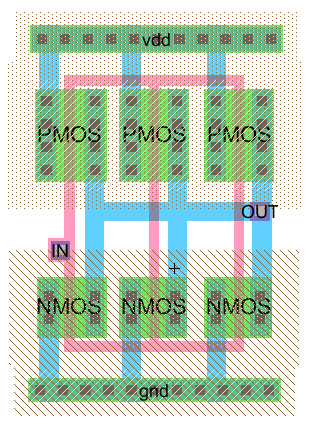
\includegraphics[scale=0.6]{./FO4_l.png}
    \rule{35em}{0.5pt}
  \caption[FO4]{Layout del inversor de salida del bloque Slave}
  \label{fig:FO4_l}
\end{figure}

\subsection{Circuito completo}

Las conexiones de los módulos mencionados en secciones anteriores y que en conjunto forman el flip-flop Master-Slave para 1 bit es el mostrado en la figura \ref{fig:Completo}. Se puede observar que para las conexiones se utilizó únicamente Metal 2

\begin{figure}[htbp]
  \centering
    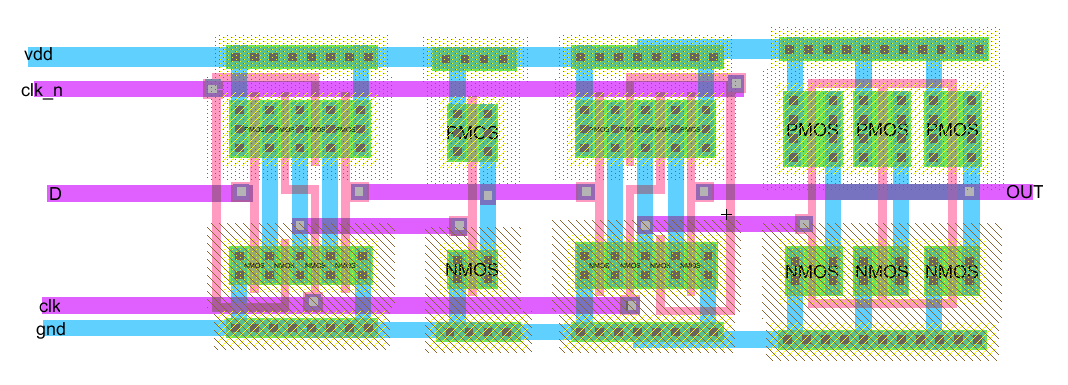
\includegraphics[scale=0.6]{./Completo.png}
    \rule{35em}{0.3pt}
  \caption[Completo]{Layout del circuito completo del Flip-Flop para 1 bit}
  \label{fig:Completo}
\end{figure}




\section{Simulación para caracterización del Flip-Flop}



\section{Análisis de datos y resultados.}






\section{Conclusiones.}
\begin{itemize}
\item Los retardos de fall son mas lentos que los de rise, debido a la movilidad de los portadores presentes en cada red.
\item En el diseño de una compuerta, el método de esfuerzo lógico es necesario para poder dimensionar los transistores, mientras que el método de Elmore permite el análisis de los casos de delay de la compuerta.
\item La teoría del esfuerzo lógico y sus cálculos nos dán una buena aproximación para determinar una buena aproximación con los tiempos de retardo
\item Las técnicas de los caminos de Euler y el diseño del diagrama de palitos llega a ser muy útil para la creación de los layouts.

\end{itemize}

\section{Bibliografía}
%----------------------------------------------------------------------------------------
\begin{thebibliography}{3}

\bibliographystyle{unsrtnat} % Use the "unsrtnat" BibTeX style for formatting the Bibliography

\bibitem[Wey(1999)]{Wey1999}
[1] N. Weste, D. Harris. 
\newblock {CMOS VLSI Design: A Circuits and Systems Perspective , 4 edition.}.
\newblock \emph{Boston: Addison-Wesley}, 2010.

\bibitem[Wey(1999)]{Wey1999}
[2] J. Rabaey, A. Chandrakasan y B. Nikolic. 
\newblock { Digital Integrated Circuits: A Design Perspective.}.
\newblock \emph{Prentice Hall}, 2005.

\bibitem[Wey(1999)]{Wey1999}
[3]Test Data .On SemiconductorC5.Mosis. Recompilado de:
\newblock \emph{http://www.ie.itcr.ac.cr/achacon/ \\* Intro$\_Diseno\_CI/Modelos\_Spice\_$MOSIS/v03m-params.txt}, el 07/09/2015

\end{thebibliography}

\end{document}